\documentclass{standalone}
\usepackage{tikz}
\usetikzlibrary{patterns}
\usetikzlibrary{positioning}
\usetikzlibrary{patterns, positioning}
\usetikzlibrary{shapes.misc}
\usepackage[outline]{contour}
\contourlength{1.5pt} 
\usepackage[sfdefault]{ClearSans}

\begin{document}
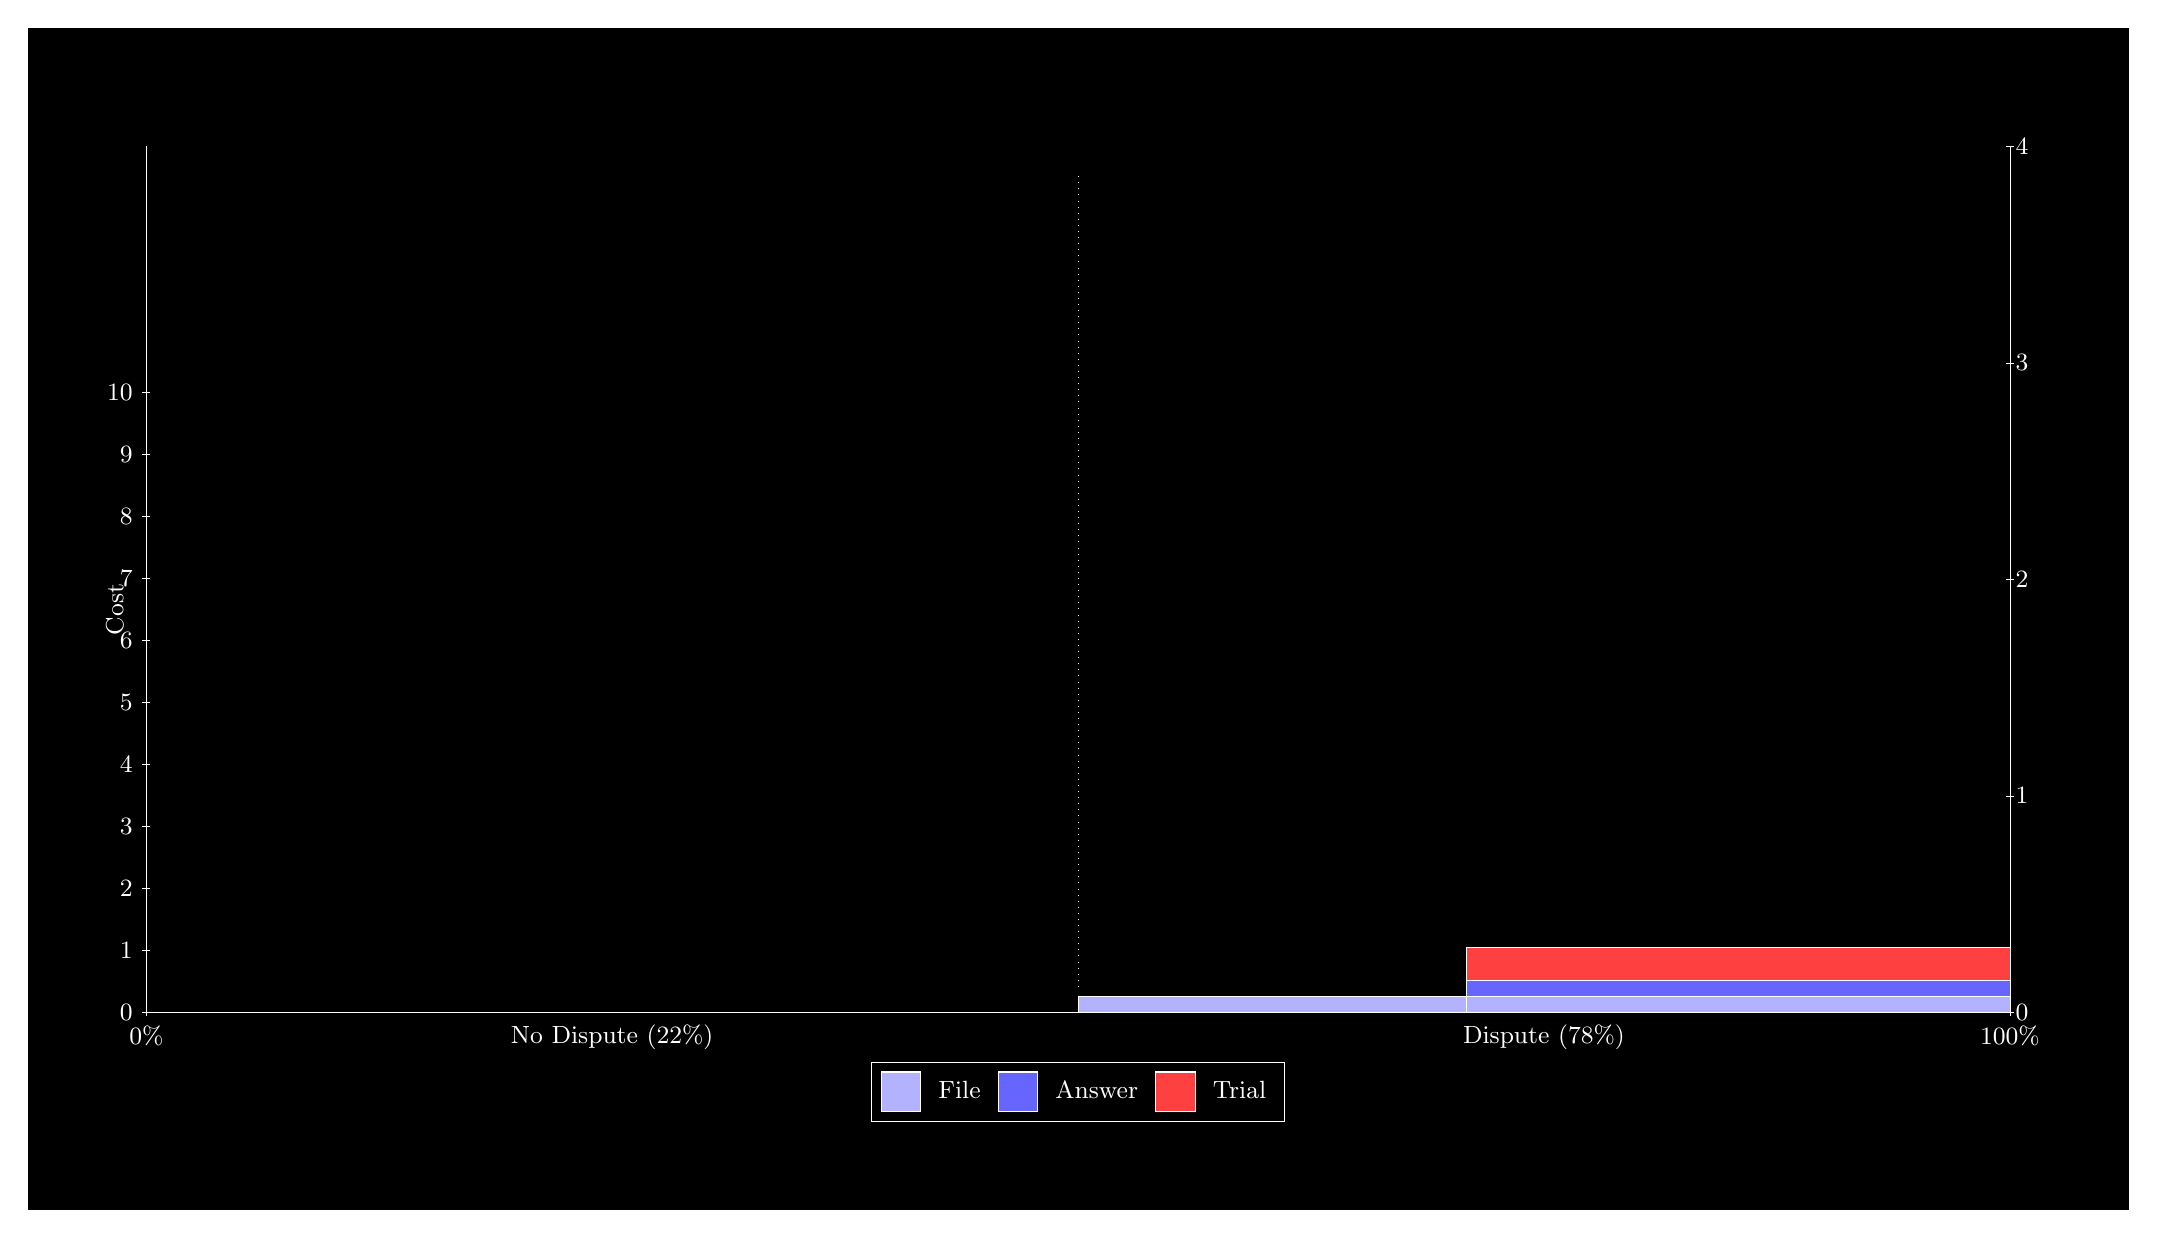
\begin{tikzpicture}
\draw[fill=black] (0,0) rectangle (26.667,15);
\draw[fill=blue!30,draw=white,very thin] (13.333,2.5) rectangle (18.265,2.7063);
\draw[fill=blue!30,draw=white,very thin] (18.265,2.5) rectangle (25.167,2.7063);
\draw[fill=blue!60,draw=white,very thin] (18.265,2.7063) rectangle (25.167,2.9125);
\draw[fill=red!75,draw=white,very thin] (18.265,2.9125) rectangle (25.167,3.325);
\draw[white,very thin] (1.5,2.5) -- (1.5,13.5);
\node[font=\small,rotate=90,text=white, anchor=center] at (1.1, 7.6195) {Cost};
\draw[white,very thin] (1.45,2.5) -- (1.55,2.5);
\node[font=\small,text=white, anchor=east] at (1.45, 2.5) {0};
\draw[white,very thin] (1.45,3.2876) -- (1.55,3.2876);
\node[font=\small,text=white, anchor=east] at (1.45, 3.2876) {1};
\draw[white,very thin] (1.45,4.0752) -- (1.55,4.0752);
\node[font=\small,text=white, anchor=east] at (1.45, 4.0752) {2};
\draw[white,very thin] (1.45,4.8628) -- (1.55,4.8628);
\node[font=\small,text=white, anchor=east] at (1.45, 4.8628) {3};
\draw[white,very thin] (1.45,5.6505) -- (1.55,5.6505);
\node[font=\small,text=white, anchor=east] at (1.45, 5.6505) {4};
\draw[white,very thin] (1.45,6.4381) -- (1.55,6.4381);
\node[font=\small,text=white, anchor=east] at (1.45, 6.4381) {5};
\draw[white,very thin] (1.45,7.2257) -- (1.55,7.2257);
\node[font=\small,text=white, anchor=east] at (1.45, 7.2257) {6};
\draw[white,very thin] (1.45,8.0133) -- (1.55,8.0133);
\node[font=\small,text=white, anchor=east] at (1.45, 8.0133) {7};
\draw[white,very thin] (1.45,8.8009) -- (1.55,8.8009);
\node[font=\small,text=white, anchor=east] at (1.45, 8.8009) {8};
\draw[white,very thin] (1.45,9.5885) -- (1.55,9.5885);
\node[font=\small,text=white, anchor=east] at (1.45, 9.5885) {9};
\draw[white,very thin] (1.45,10.376) -- (1.55,10.376);
\node[font=\small,text=white, anchor=east] at (1.45, 10.376) {10};

\draw[white,dotted,very thin] (13.333,2.83) -- (13.333,13.17);
\draw[white,very thin] (25.167,2.5) -- (25.167,13.5);
\draw[white,very thin] (25.117,2.5) -- (25.217,2.5);
\node[font=\small,text=white, anchor=west] at (25.117, 2.5) {0};
\draw[white,very thin] (25.117,5.25) -- (25.217,5.25);
\node[font=\small,text=white, anchor=west] at (25.117, 5.25) {1};
\draw[white,very thin] (25.117,8) -- (25.217,8);
\node[font=\small,text=white, anchor=west] at (25.117, 8) {2};
\draw[white,very thin] (25.117,10.75) -- (25.217,10.75);
\node[font=\small,text=white, anchor=west] at (25.117, 10.75) {3};
\draw[white,very thin] (25.117,13.5) -- (25.217,13.5);
\node[font=\small,text=white, anchor=west] at (25.117, 13.5) {4};

\draw[white,very thin] (1.5,2.5) -- (25.167,2.5);
\draw[white,very thin] (1.5,2.45) -- (1.5,2.55);
\node[font=\small,text=white, anchor=north] at (1.5, 2.45) {0\%};
\draw[white,very thin] (25.167,2.45) -- (25.167,2.55);
\node[font=\small,text=white, anchor=north] at (25.167, 2.45) {100\%};

\node[font=\small,text=white,anchor=south] at (7.4167, 1.9) {No\ Dispute\ (22\%)};
\node[font=\small,text=white,anchor=south] at (19.25, 1.9) {Dispute\ (78\%)};
\draw (13.3333,2.5) node (B) {};
\begin{scope}[align=center]
\matrix[scale=0.5,draw=white,below=0.5cm of B,nodes={draw},column sep=0.1cm]{
\node[rectangle,draw,minimum width=0.5cm,minimum height=0.5cm,fill=blue!30]{}; & \node[draw=none,font=\small,text=white]{File}; &
\node[rectangle,draw,minimum width=0.5cm,minimum height=0.5cm,fill=blue!60]{}; & \node[draw=none,font=\small,text=white]{Answer}; &
\node[rectangle,draw,minimum width=0.5cm,minimum height=0.5cm,fill=red!75]{}; & \node[draw=none,font=\small,text=white]{Trial}; \\\\
};\end{scope}

\end{tikzpicture}
\end{document}